\documentclass[20pt]{beamer}
\usepackage{graphicx} % Required for inserting images
\usepackage{tikz}%for figures
\usepackage{adjustbox}
\usepackage{subfig}
\usepackage{pgfplots}\pgfplotsset{compat=1.9}
\usepackage{pgfplots}
\usepackage{amsmath}
\usepackage{amsthm} %theorems
\usepackage{amsfonts}
\usepackage{amssymb} %lesssim, etc
\usepackage{algorithm}
\usepackage[noend]{algpseudocode}
\usepackage{natbib}
\usepackage{bbm}

\usepackage{bbm}
\usepackage{xcolor}
\usepackage{hyperref}[] % hyperlink
\hypersetup{
colorlinks = true,
linkcolor = blue, %Colour of internal links
filecolor = magenta,
urlcolor = blue, %Colour for external hyperlinks
citecolor = blue, %Colour of citations
pdfpagemode=UseOutlines
}

\newcommand{\jongmin}[1]{
{ \color{blue} Jongmin: #1}
}

\newcommand\numberthis{\addtocounter{equation}{1}\tag{\theequation}}
\newtheorem{thm}{Theorem}[section]
\newtheorem{prop}[thm]{Proposition}
\newtheorem{lem}[thm]{Lemma}
\newtheorem{cor}[thm]{Corollary}


%%
%% If some other type is need, say conjectures, then it is constructed
%% by editing and uncommenting the following.
%%
\theoremstyle{definition}
\newtheorem{conj}{Conjecture}
\newtheorem{alg}{Algorithm} 
%Information to be included in the title page:
\title{Exact spike train inference via $\ell_0$ optimization}


\begin{document}

\begin{frame}
	\large
$\ell_0$ Neural Spike Train Inference via Tight Convexification
	\small
	\begin{itemize}
		\item 	presenter: Jongmin Mun 
		\item Final presentation for USC ISE-617 2026
	\end{itemize}

	
\end{frame}


\begin{frame}
	\tableofcontents
\end{frame}

\section{Why analyze spike trains?}
\begin{frame}

	\begin{itemize}
\item Neural spike train
\item Why do we analyze them
		\end{itemize}
\end{frame}

\begin{frame}
\begin{figure}
	\centering
	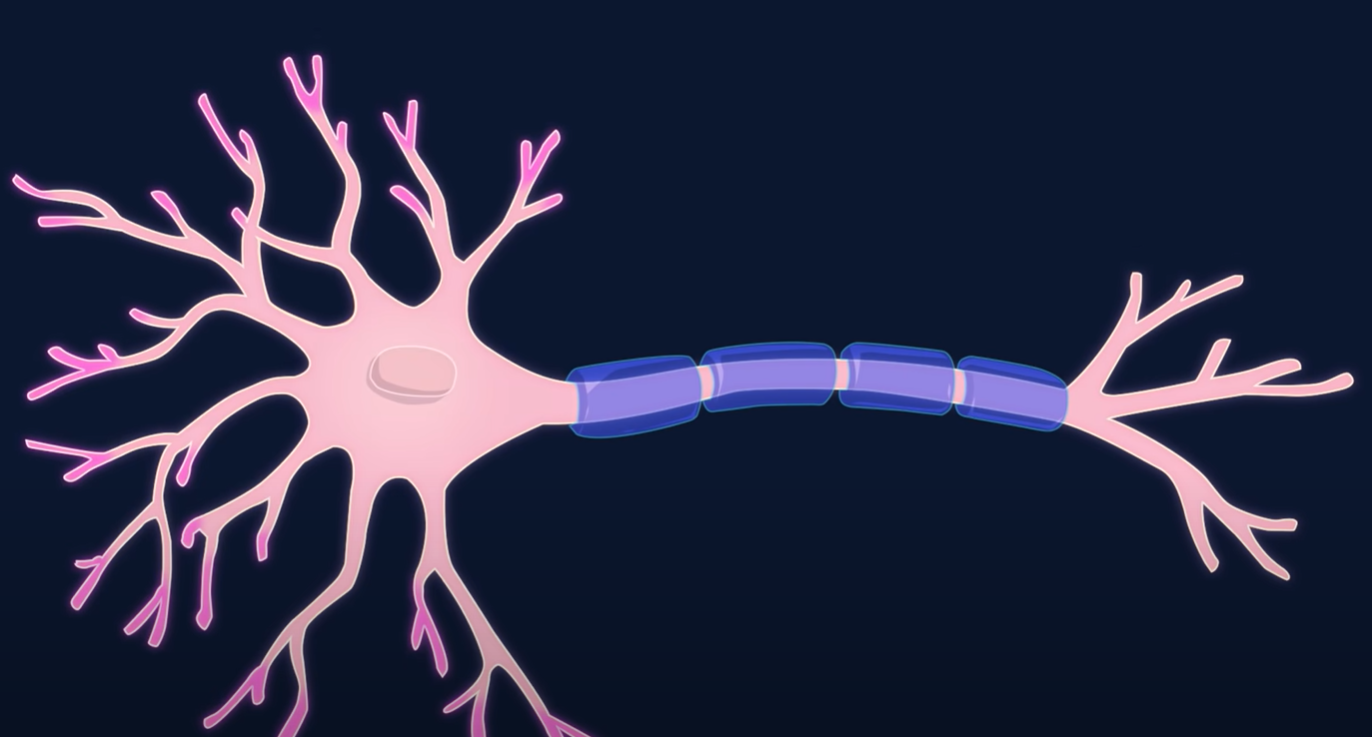
\includegraphics[width=0.9\linewidth]{neuron}
	\caption{Neurons receive, process, and transmit information through a phenomenon called action potential}
	\label{fig:neuron}
\end{figure}
	\begin{figure}
	\centering
	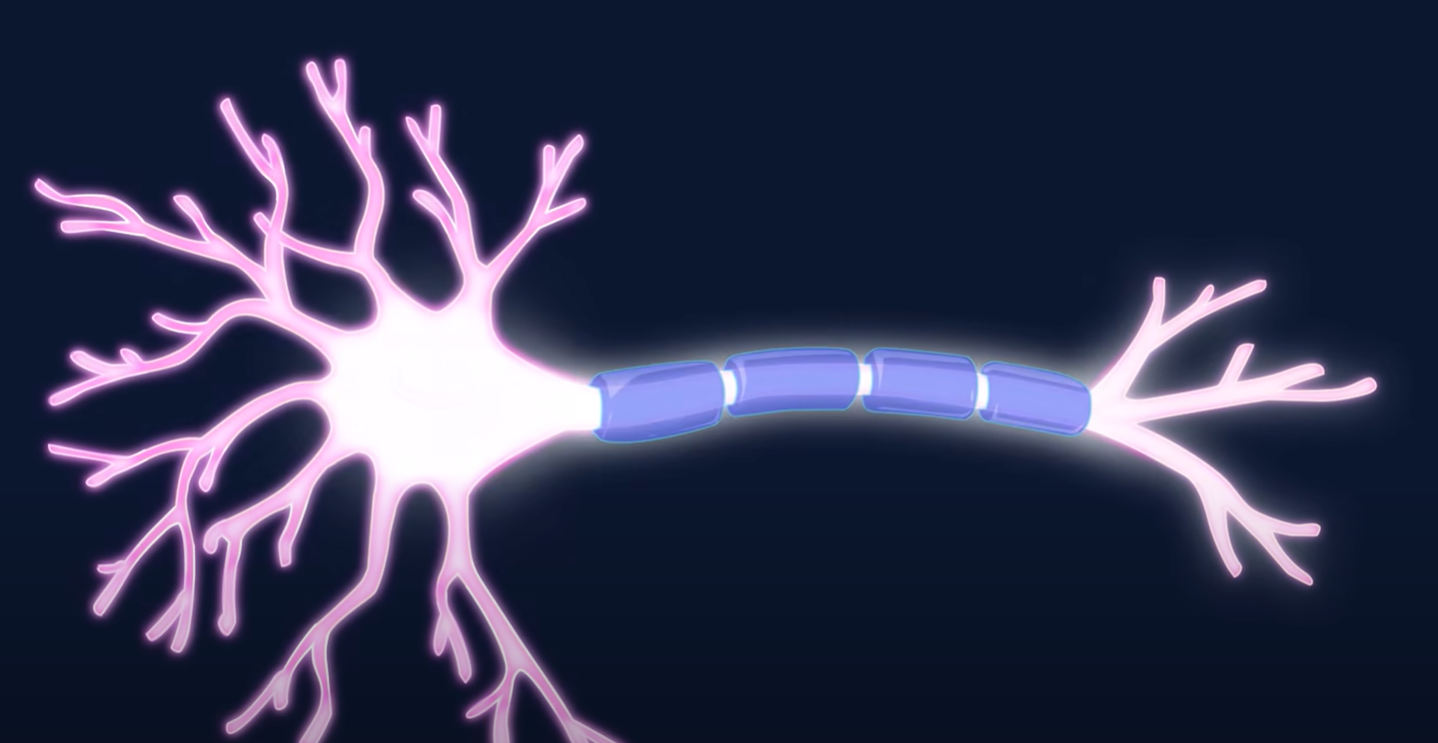
\includegraphics[width=0.9\linewidth]{neuron_fire}
	\caption{When action potential happens, we say the the neuron fires. }
	\label{fig:neuron_fire}
\end{figure}

\end{frame}


\begin{frame}

\end{frame}

\begin{frame}
	\begin{figure}
		\centering
		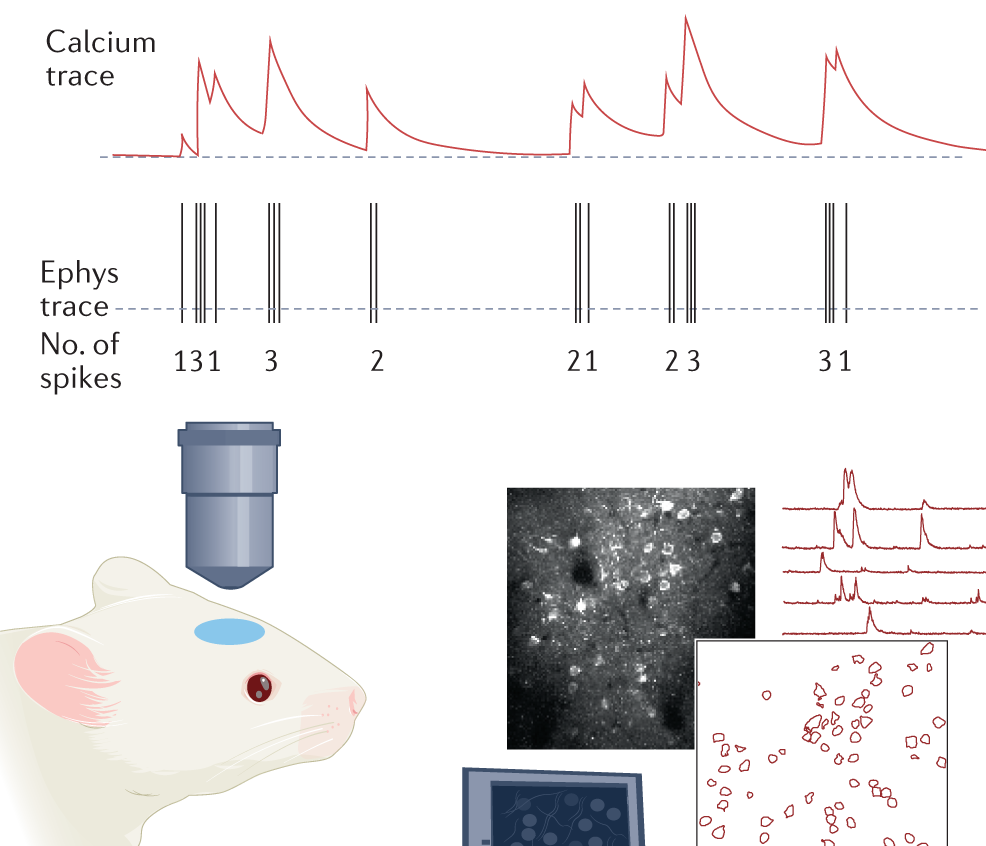
\includegraphics[width=0.7\linewidth]{spikeTrain}
		\caption{Calcium imaging records the action potentials - spike train.}
		\label{fig:neuron_fire}
	\end{figure}
\end{frame}

\begin{frame}
		\frametitle{Binary encoding}
		\begin{itemize}
			\item In the spike train, the information is encoded in whether a neuron fires or not, rather than in the magnitude of the potential.
			\item ALL neural activities (your thoughts, orders for your action) are encoded this way.
		\end{itemize}


\end{frame}

\begin{frame}
	\frametitle{Two research tasks}
	\begin{itemize}
		\item 	  
	Neural decoding: mind-reading
		
		\item Neural encoding: animal control
	\end{itemize}
		All  require accurate spike train inference.
	Recordings are always noisy.

\end{frame}

\begin{frame}
	How can we better detect the spikes?
	\frametitle{Two ways to improve}
	\begin{itemize}
		\item 	   Develop new recording technology
		
		\item Improve the detection algorithms (this paper)
	\end{itemize}

	
\end{frame}

\section{Contributions}
\begin{frame}
	\frametitle{Contributions}
\begin{itemize}
	\item Formulates the spike detection as $\ell_0$ regularized optimization
	\item Transforms the problem in to change-point detection problem
	\item Devise an $O(T^2)$ solver based on dynamic programming
	\item Faster and more accurate than $\ell_1$ regularization.
	\end{itemize}
\end{frame}

\section{Model}
\begin{frame}
	\frametitle{Three stages of models}
\begin{itemize}
	\item Spike sequence (fixed, unobserved)
	\item Underlying calcium concentration process (fixed, unobserved)
	\item Noise-added observations (random, observed)
\end{itemize}
\end{frame}
%
%
\begin{frame}
	\frametitle{1. Spike sequence}

\( s_t \geq 0 \), $t  1, \ldots, T$
	\begin{itemize}
		\item Example: \( 0,\, 3.5,\, 0,\, 0,\, 1.1,\, 0,\, 0,\, 2,\, \dots \)
		\item If \( s_t > 0 \): spike at time \( t \)
		\item If \( s_t = 0 \): no spike at time \( t \)
		\item Fixed unknown parameter of interest
		\item Sparsity assumption
\end{itemize}

\end{frame}


%
\begin{frame}
	\frametitle{2. Underlying calcium concentration}

	\begin{itemize}
		\item First-order autoregressive process
		\[
		C_t = \gamma C_{t-1} + s_t, \quad t = 2, 3, \dots, T
		\]
		\item Spike appears abrupt, and gradually disappears. 
		\item The effect of spikes can overlap
		\item Fixed unknown parameter
	\end{itemize}

	\end{frame}
	%
	
\begin{frame}

	\begin{figure}
	\centering
	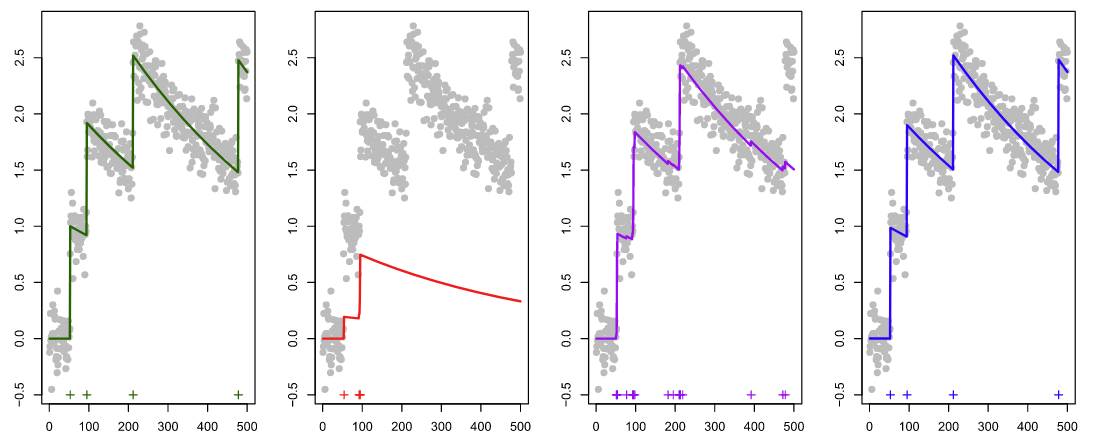
\includegraphics[width=0.9\linewidth]{calcium}
	\caption{ Spike appears abrupt, and gradually disappears}
	\label{fig:neuron_fire}
\end{figure}

	
		
	\end{frame}
	
	
	\begin{frame}
		\frametitle{3. Observed fluorescence process}
	\[
	Y_t = c_t + \varepsilon_t, \quad \varepsilon_t \sim_{\text{ind}} (0, \sigma^2)
	\]
	\\
	$\text{for} \quad t = 1, \ldots, T$
\end{frame}

\section{Optimization problem}
\begin{frame}
	\frametitle{Optimization problem}
\small
\begin{align*}
	\min_{c_1, \ldots, c_T,\, s_2, \ldots, s_T}~& \frac{1}{2} \sum_{t=1}^T (y_t - c_t)^2 + \lambda \sum_{t=2}^T 
	\mathbbm{1}(s_t = 0) \\
	\text{s.t.}~& s_t = c_t - \gamma c_{t-1}.
\end{align*}
\begin{itemize}
	\item Regularization $\lambda \mathbbm{1}(c_t \neq \gamma c_{t-1})$ ties $c_t$ and $c_{t+1}$.
	\item This tie is active only when $c_t = \gamma C_{t-1}$ ($s_t = 0$) (no spike)
\end{itemize}


\end{frame}

\begin{frame}
	\frametitle{Another viewpoint}

		Thus, if the solution sets $s_t > 0$, than we actually solved the problem that decouples into $[1, t-1]$ and $[t+1, T]$, and $t$ is a changepoint.

\end{frame}


\begin{frame}

Thus, problem is equivalent to the changepoint detection problem:
\[
\text{(spike magnitude} \;\longleftrightarrow\; \text{timepoint)}
\]
\[
\begin{array}{ccccccccc}
	0 & 1.1 & 0 & 0 & 3.5 & 0 & 2.33 & \cdots \\
	& 2 &  &  & 5 &  & 8 & 
\end{array}
\]

 
\end{frame}

\begin{frame}
	\frametitle{Proposition 1}
	\small
The problem is equivalent to
\begin{equation*}
	\min_{0 = \tau_0 < \tau_1 < \cdots < \tau_k < \tau_{k+1} = T} 
	\left\{ \sum_{j=0}^k \mathcal{D}(\tau_j+1, \tau_{j+1}) + \lambda k \right\}.
\end{equation*}
for two timepoints $a = \tau_j + 1, \quad b = \tau_{j+1}$,
\begin{align*}
\mathcal{D}(a,b) := &\arg\min_{c_a, c_{a+1}, \ldots, c_b} \frac{1}{2} \sum_{t=a}^b (y_t - c_t)^2\\& \text{s.t.} \quad c_t = \gamma c_{t-1}.
\end{align*}

	\end{frame}
\begin{frame}
\begin{align*}
	\mathcal{D}(a,b) := &\arg\min_{c_a, c_{a+1}, \ldots, c_b} \frac{1}{2} \sum_{t=a}^b (y_t - c_t)^2\\& \text{s.t.} \quad c_t = \gamma c_{t-1}.
\end{align*}
\begin{itemize}
	\item Measures homogeneity of the measurement
	\item Has a closed-form formula (Proposition 2).
\end{itemize}
%
\end{frame}
%
\begin{frame}
	\small
	\begin{equation*}
		\min_{0 = \tau_0 < \tau_1 < \cdots < \tau_k < \tau_{k+1} = T} 
		\left\{ \sum_{j=0}^k \mathcal{D}(\tau_j+1, \tau_{j+1}) + \lambda k \right\}.
	\end{equation*}
Find not too many timepoints such that  
between two consecutive timepoints, the measurements are homogeneous
\end{frame}

\section{$O(T^2)$ algorithm}
\begin{frame}
Apply the dynamic programming algorithm proposed by Jackson et al.\ (2005, \textit{IEEE Signal Processing Letters}) developed for changepoint detection.

\end{frame}

\begin{frame}
	\footnotesize
	\[
	F(T) := \min_{\substack{0 = \tau_0 < \tau_1 < \cdots < \tau_k < \tau_{k+1} = T}} 
	\left\{ 
	\underbrace{
		\sum_{j=0}^{k} \mathcal{D}(\tau_j+1, \tau_{j+1}) + \lambda k
	}_{\text{(A)}}
	\right\}
	\quad \text{($k$ intervals)}
	\]
	
	\[
	\text{(A)} =
	\sum_{j=0}^{k} \left[ \mathcal{D}(\tau_j+1, \tau_{j+1}) + \lambda \right] - \lambda
	\quad \text{($k+1$ terms)}
	\]
	
	\[
	= \underbrace{
		\sum_{j=0}^{k-1} \left[ \mathcal{D}(\tau_j+1, \tau_{j+1}) + \lambda \right] - \lambda
	}_{\text{$\tau_0, \ldots, \tau_k$: $k$ intervals, contributes to } F(\tau_k)}
	+ \underbrace{\mathcal{D}(\tau_k+1, \tau_{k+1}) + \lambda}_{\text{$\tau_k+1, \tau_{k+1}$}}
	\]
\end{frame}


\begin{frame}
	\frametitle{Dynamic programming}
	\small
Set $F(0) = -\lambda$ 

\[
F(1) = \min_{\tau \in \{0\}} \left\{ F(\tau) + \mathcal{D}(y_{\tau+1:1}) + \lambda \right\} 
\]
\[
F(2) = \min_{\tau \in \{0,1\}} \left\{ F(\tau) + \mathcal{D}(y_{\tau+1:2}) + \lambda \right\}
\]
$\mathcal{D}$ calculation in constant time, at  step $t$, reads  $t$ data: $O(\sum_{t=1}^T T) = O(T^2)$
\end{frame}

\section{Conclusion}
\begin{frame}
	\begin{itemize}
		\item Formulates the spike detection as $\ell_0$ regularized optimization
		\item Transforms the problem in to change-point detection problem
		\item Devise an $O(T^2)$ solver based on dynamic programming
		\item Faster and more accurate than $\ell_1$ regularization (numerically).
		\item No statistical theory, just optimization
	\end{itemize}
\end{frame}

%
%

\bibliographystyle{apalike}
\bibliography{reference}
\end{document}